% This is samplepaper.tex, a sample chapter demonstrating the
% LLNCS macro package for Springer Computer Science proceedings;
% Version 2.21 of 2022/01/12
%
\documentclass[runningheads]{llncs}
%
\usepackage[T1]{fontenc}
\usepackage{graphicx}
% T1 fonts will be used to generate the final print and online PDFs,
% so please use T1 fonts in your manuscript whenever possible.
% Other font encondings may result in incorrect characters.
%
\usepackage{graphicx}
% Used for displaying a sample figure. If possible, figure files should
% be included in EPS format.
%
% If you use the hyperref package, please uncomment the following two lines
% to display URLs in blue roman font according to Springer's eBook style:
%\usepackage{color}
%\renewcommand\UrlFont{\color{blue}\rmfamily}
%

% jiayuan for math and algorithm
\usepackage{amsmath}
\usepackage{amssymb}
\usepackage{algorithm}  % for algorithms
\usepackage{algorithmic}

\begin{document}
%
\title{CS6216 Project Report}
%
%\titlerunning{Abbreviated paper title}
% If the paper title is too long for the running head, you can set
% an abbreviated paper title here
%
\author{Apivich Hemachandra\inst{1}\orcidID{0000-1111-2222-3333} \and
Jiashu Tao\inst{1}\orcidID{A0159714X} \and
Bo Wang\inst{1}\orcidID{2222--3333-4444-5555}   \and
Jiayuan Ye\inst{1} }
%
\authorrunning{F. Author et al.}
% First names are abbreviated in the running head.
% If there are more than two authors, 'et al.' is used.
%
\institute{School of Computing, National University of Singapore, Singapore }
%
\maketitle              % typeset the header of the contribution
%
\begin{abstract}
We reproduce the Stein Variational Gradient Descent (SVGD) algorithm proposed by Liu et al [1]. Similar to gradient descent, SVGD is a variational inference algorithm that iterative optimizes a set of particles to match a distribution by applying functional gradient descent. In this project, we reproduce the algorithm with the help of some publicly available code bases and verify the experimental results in the paper. 

\end{abstract}
\section{Introduction}
\subsection{A Subsection Sample}
Please note that the first paragraph of a section or subsection is
not indented. The first paragraph that follows a table, figure,
equation etc. does not need an indent, either.

Subsequent paragraphs, however, are indented.

\subsubsection{Sample Heading (Third Level)} Only two levels of
headings should be numbered. Lower level headings remain unnumbered;
they are formatted as run-in headings.

\paragraph{Sample Heading (Fourth Level)}
The contribution should contain no more than four levels of
headings. Table~\ref{tab1} gives a summary of all heading levels.

\begin{table}
\caption{Table captions should be placed above the
tables.}\label{tab1}
\begin{tabular}{|l|l|l|}
\hline
Heading level &  Example & Font size and style\\
\hline
Title (centered) &  {\Large\bfseries Lecture Notes} & 14 point, bold\\
1st-level heading &  {\large\bfseries 1 Introduction} & 12 point, bold\\
2nd-level heading & {\bfseries 2.1 Printing Area} & 10 point, bold\\
3rd-level heading & {\bfseries Run-in Heading in Bold.} Text follows & 10 point, bold\\
4th-level heading & {\itshape Lowest Level Heading.} Text follows & 10 point, italic\\
\hline
\end{tabular}
\end{table}


\noindent Displayed equations are centered and set on a separate
line.
\begin{equation}
x + y = z
\end{equation}
Please try to avoid rasterized images for line-art diagrams and
schemas. Whenever possible, use vector graphics instead (see
Fig.~\ref{fig1}).


\begin{theorem}
This is a sample theorem. The run-in heading is set in bold, while
the following text appears in italics. Definitions, lemmas,
propositions, and corollaries are styled the same way.
\end{theorem}
%
% the environments 'definition', 'lemma', 'proposition', 'corollary',
% 'remark', and 'example' are defined in the LLNCS documentclass as well.
%
\begin{proof}
Proofs, examples, and remarks have the initial word in italics,
while the following text appears in normal font.
\end{proof}
For citations of references, we prefer the use of square brackets
and consecutive numbers. Citations using labels or the author/year
convention are also acceptable. The following bibliography provides
a sample reference list with entries for journal
articles~\cite{ref_article1}, an LNCS chapter~\cite{ref_lncs1}, a
book~\cite{ref_book1}, proceedings without editors~\cite{ref_proc1},
and a homepage~\cite{ref_url1}. Multiple citations are grouped
\cite{ref_article1,ref_lncs1,ref_book1},
\cite{ref_article1,ref_book1,ref_proc1,ref_url1}.

\subsubsection{Acknowledgements} Please place your acknowledgments at
the end of the paper, preceded by an unnumbered run-in heading (i.e.
3rd-level heading).
\section{Summary of the Paper}

The paper proposes a general-purpose variational inference algorithm -- Stein Variation Gradient Descent (SVGD). In this section, we summarize the author's justification for the design of the SVGD algorithm. The pseudocode is in Algorithm \ref{alg:svgd}. The ultimate goal of the SVGD algorithm is to perform inference on a target distribution $p(x)$ on $\mathcal{X}=\mathbb{R}^d$, i.e. to estimate $\mathbb{E}_{x\sim p(x)}[f(x)]$ for some function $f(x)$, or to estimate the shape of the distribution $p(x)$. To do that, the algorithm constructs and updates multiple particles $x_1, \cdots, x_n$, which approximates a distribution $q(x)$ that has small KL divergence with regard to the target distribution $p(x)$. More specifically, they aim to solve the following problem.

% We first summarize the author's justification for the design of the SVGD algorithm, and then explain the extreme case, scalability, and performance of the SVGD algorithm.

% \subsection{Design of SVGD}

\begin{algorithm}[t!]
	\caption{Bayesian Inference via Variational Gradient Descent~\cite{ref_article_svgd}}
	\label{alg:svgd}
	\begin{algorithmic}
		\STATE {\bfseries Input:} A target distribution with density function $p(x)$ and a set of initial particles $\{x_i^0\}_{i=1}^n$.
		\STATE{\bfseries Output:} A set of particles $\{x_i\}_{i=1}^n$ that approximates the target distribution.
		\FOR {iteration $\ell$}
		\STATE{$x_i^{\ell+1}\leftarrow x_i^l + \epsilon_l \hat{\mathbf{\phi}}^*(x_i^\ell)$,
		
		where $\hat{\mathbf{\phi}}^*(x) = \frac{1}{n} \sum_{j=1}^n\left[ k(x_{j}^\ell, x)\nabla_{x_j^\ell}\log p(x_j^\ell) + \nabla_{x_j^\ell} k(x_j^\ell, x)\right]$}
		\ENDFOR
	\end{algorithmic}
\end{algorithm}

\begin{align}
    x_1,\cdots,x_n\sim q(x), \text{ where }q(x) = \arg\min_{q(x)} KL(q(x)\lVert p(x)).
\end{align}

The algorithm is designed with the following key ingredients.

\begin{enumerate}
    \item Iterative Particle Movement: under a small particle movement $T(x) = x + \epsilon \mathbf{\phi}(x)$, the transformed particles follow a push-forward distribution $q_{[\epsilon\mathbf{\phi}]}(x) = T_{\#}q(x)$ that captures the distribution of $T(x)$ for $x\sim q(x)$. Here $\epsilon$ is a small stepsize, and $\phi(x): \mathbb{R}^d\rightarrow \mathbb{R}^d$ could be any smooth mapping.
    \item Steepest descent direction and Stein's discrepancy: to find the mapping $\mathbf{\phi}(x)$ that results in the steepest descent of KL divergence, the author translate this objective to be the following Stein's discrepancy,
    \begin{align}
    \label{eqn:objective}
         \arg\max_\phi\frac{d}{d \epsilon}KL(q_{[\epsilon\mathbf{\phi}]}\left(x)\lVert p(x)\right) = \arg\max_\phi \mathbb{E}_{x\sim q}\left[trace\left(\mathcal{A}_p \mathbf{\phi}(x)\right)\right]
    \end{align}
    where the operator $\mathcal{A}_p \phi(x)= \nabla \log p(x) \cdot \phi(x) + \nabla\phi(x)$.
    \item Kernel trick for closed form solution: Let $\mathcal{H}$ be a reproducing kernel Hilbert space with positive definite kernel $k(x,x')$, i.e. $\mathcal{H}$ is the closure of the linear span $\{f: f = \sum_{i=1}^m a_i \cdot k(x, x_i), a_i\in \mathbb{R}, m\in \mathbb{N}, x_i\in \mathcal{X}=\mathbb{R}^d \}$. Then for $\phi(x) = \left(\phi_1(x), \phi_2(x), \cdots, \phi_d(x)\right)^T \in \mathcal{H}^d$, s.t. $\lVert\phi\rVert_{\mathcal{H}_d}\leq S(q, p)$, \eqref{eqn:objective}  has the following closed form solution.
    \begin{align}
    \label{eqn:solution}
        \phi(x) = \mathbb{E}_{x'\sim q}\left[ \mathcal{A}_p k(x', x) \right]
    \end{align}
    where $S(q, p) = \max_{\phi\in \mathcal{H}^d, s.t. \lVert\phi\rVert_2\leq 1} \mathbb{E}_{x\sim q}\left[trace\left(\mathcal{A}_p \mathbf{\phi}(x)\right)\right]$ is the Kernelized Stein's discrepancy. Here the authors assume that the function $K(x, x')$ given fixed $x'$ lies in the stein class of target density function $p(x)$.
    \item Approximation for $\phi$ with discrete particles $x_1, \cdots, x_n$: the closed-form solution \eqref{eqn:solution} involves high dimensional integration that is often intractable. Therefore, the author uses $n$ discrete particles $x_1, \cdots, x_n$ drawn from $q$ to perform the Monte Carlo estimate for the integral. In each iteration, the particle is then updated with the estimated mapping $T = I + \epsilon \phi$.
\end{enumerate}

The summation term in the iterative update step of the algorithm can be seen to have two parts. The first term is an attractive term that tries to maximize $\log p(x)$. The second term is a repulsive term that maximizes the difference between the two points through the kernel function. Balancing the two terms allow SVGD to pick samples with high $p(x)$ but are also different from each other.

% \subsection{Extreme case of SVGD with $n=1$ particle.} 

% The SVGD algorithm under one particle is equivalent to MAP estimate under gradient descent of $\log p(x)$ where $p(x)$ is the target distribution. \footnote{This is covered in the paper authors' blog \url{https://www.cs.utexas.edu/~qlearning/project.html?p=svgd}.} For example, under the RBF kernel $k(x, x') = \frac{1}{h}e^{\lVert x- x'\rVert_2^2}$, when applying the mapping $\hat{\phi}(x)$ in Algorithm \ref{alg:svgd} to the single particle $x=x_1^\ell$, we obtain the following gradient mapping.

% \begin{align}
%     \hat{\mathbf{\phi}}^*(x)|_{x=x_1^\ell} & = k(x_1^\ell, x)|_{x=x_1^e\ll} \nabla_{x_1^\ell}\log p(x_{1}^\ell) + \nabla_{x_1^\ell}k(x_1^\ell, x)|_{x=x_1^\ell}\\
%     & = k(x_1^\ell, x_1^\ell) \nabla_{x_1^\ell}\log p(x_{1}^\ell) + \mathbf{0}\\
%     & = \frac{1}{h} \nabla_{x_1^\ell}\log p(x_{1}^\ell)
% \end{align}

% \subsection{Performance of SVGD in terms of Estimation Error}


% \subsection{Scalability of SVGD with regard to model dimension and number of particles}
\section{Experiments}
In this section, we report our reproduction effort and verification of the experimental results in the paper. For the SVGD algorithm, we test using the implementation of SVGD from the author of the original paper, and also using the implementation of the algorithm on NumPyro. The implementation on NumPyro is described further in Appendix \ref{ssect:svgd-npy}.

\subsection{Toy Example}

\newcommand{\toyfigwidth}{0.9\textwidth}
\begin{figure}[!htbp]
    \centering
    % \begin{tabular}{@{}c@{}}
    %     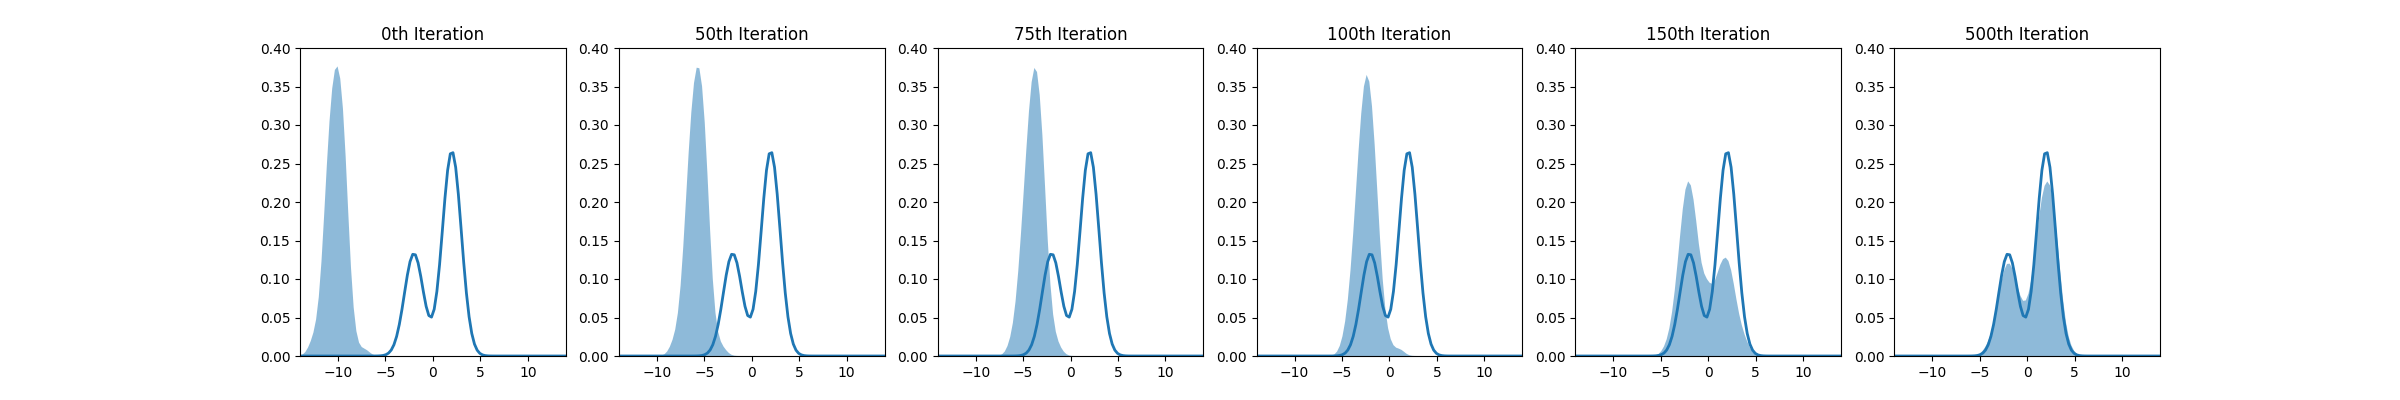
\includegraphics[width=\toyfigwidth]{figs/toy-figure1_step0.1_mu2.0_w0.33_gaussian.png} \\
    %     \small (1) StepSize = 0.1, 500 iterations, $\mu = \pm 2$, $(w_1, w_2) = (0.33, 0.67)$
    % \end{tabular}
    
    \begin{tabular}{@{}c@{}}
        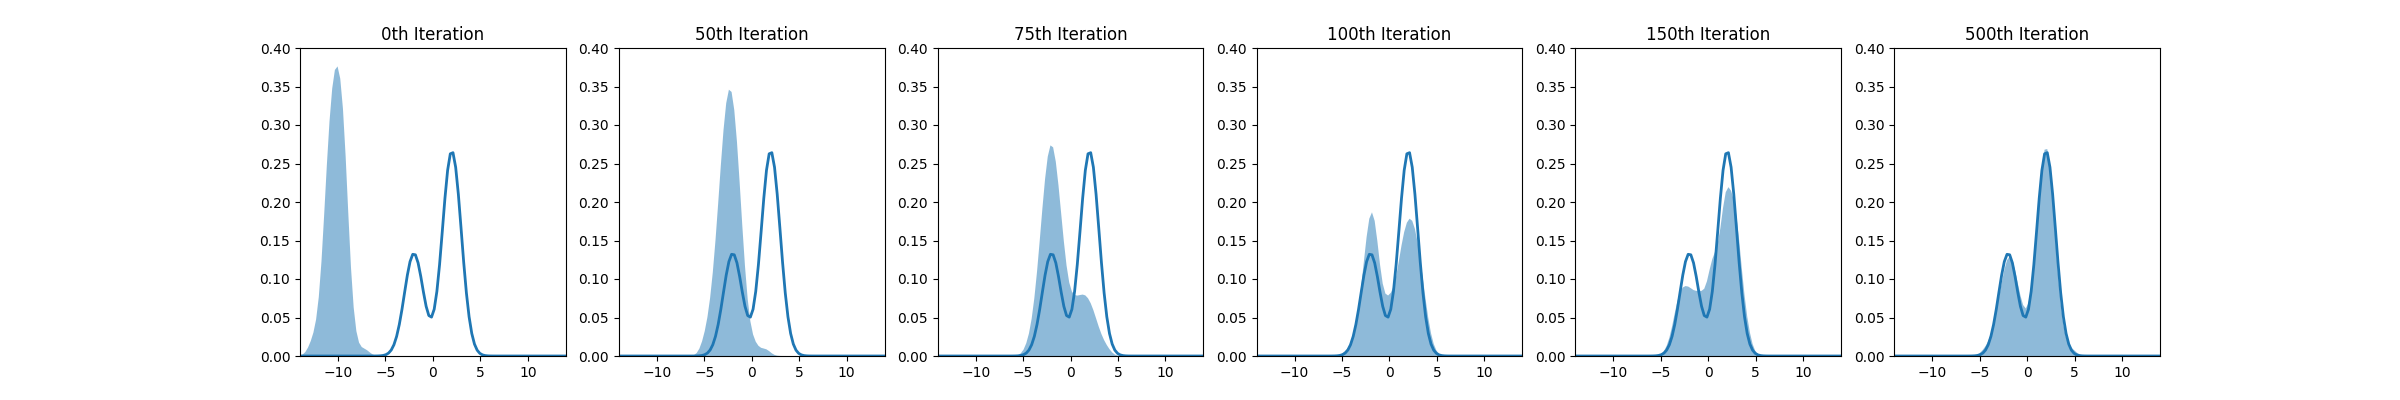
\includegraphics[width=\toyfigwidth]{figs/toy-figure1.png} \\
        \small (1) StepSize = 0.25, 500 iterations, $\mu = \pm 2$, $(w_1, w_2) = (0.33, 0.67)$
    \end{tabular}
    %\vspace{\floatsep}
    
    \begin{tabular}{@{}c@{}}
        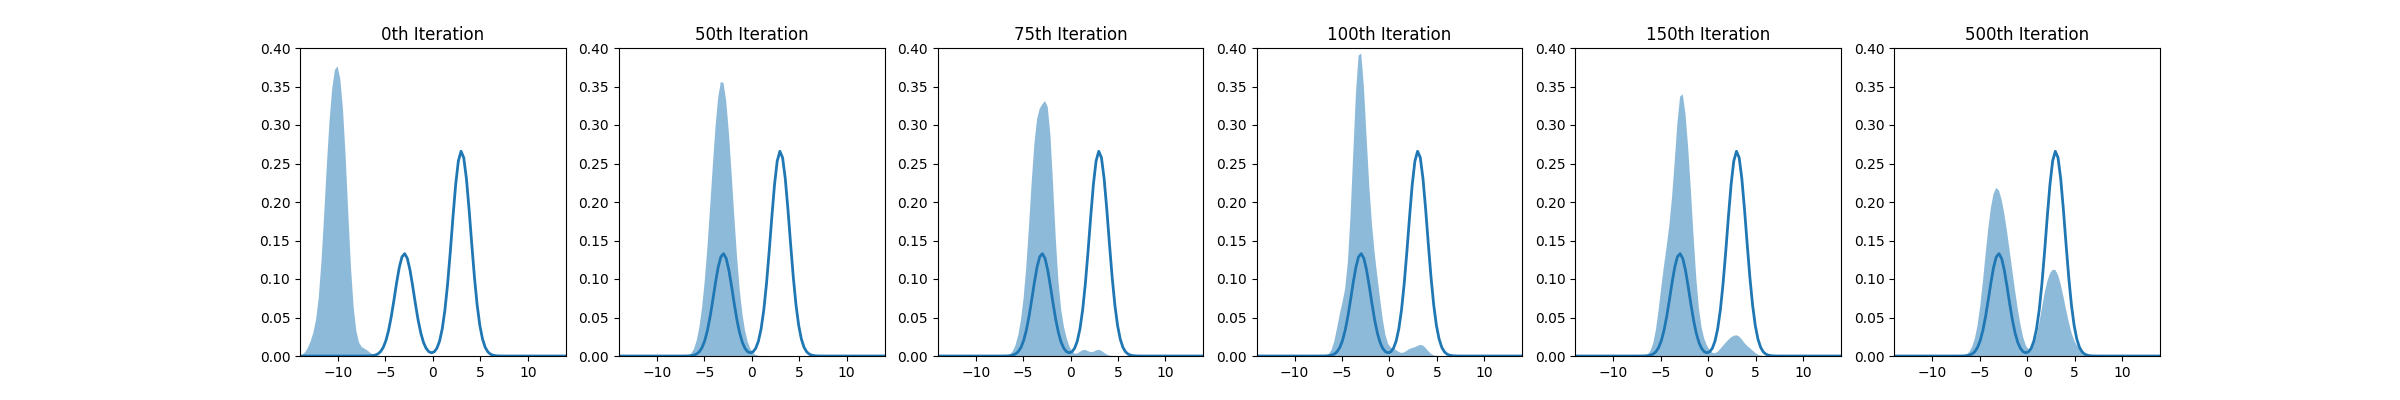
\includegraphics[width=\toyfigwidth]{figs/toy-figure1_step0.25_mu3.0_w0.33_gaussian.png} \\
        \small (2) StepSize = 0.25, 500 iterations, $\mu = \pm 3$, $(w_1, w_2) = (0.33, 0.67)$
    \end{tabular}
    
    \begin{tabular}{@{}c@{}}
        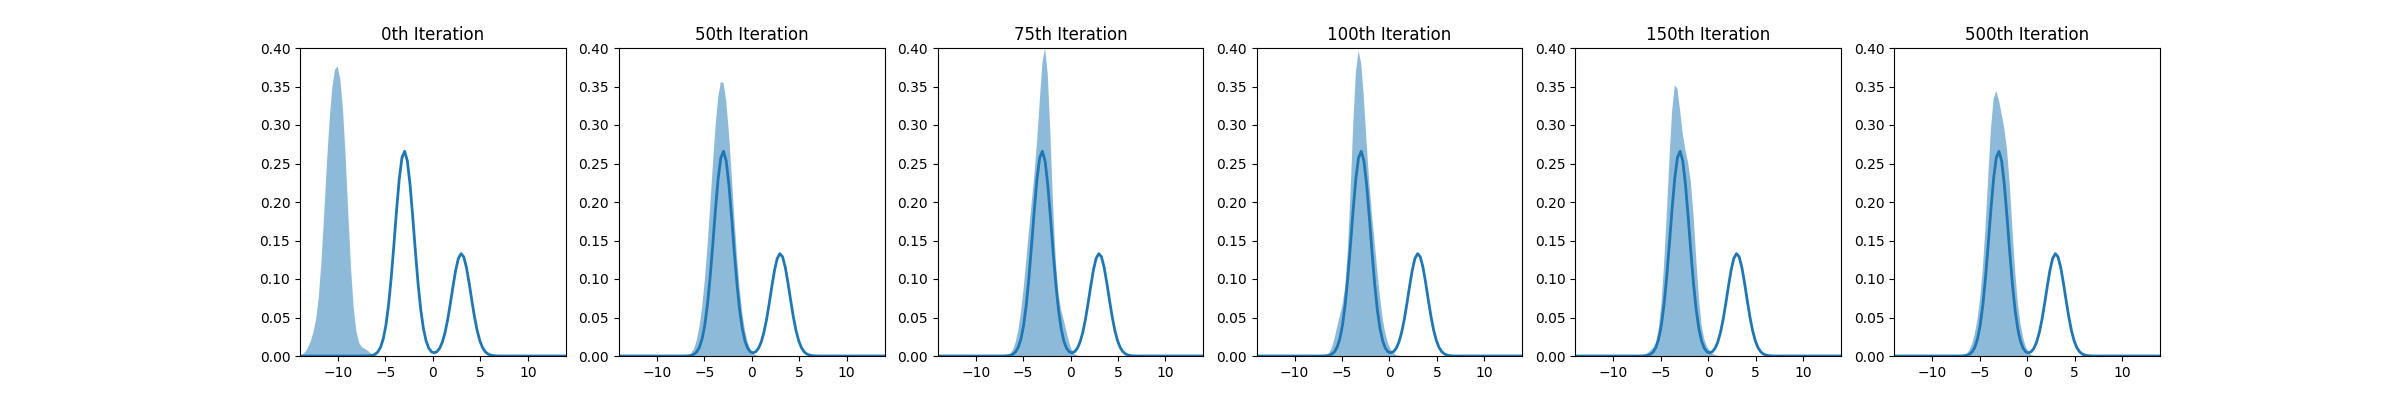
\includegraphics[width=\toyfigwidth]{figs/toy-figure1_step0.25_mu3.0_w0.67_gaussian.png} \\
        \small (3) StepSize = 0.25, 500 iterations, $\mu = \pm 3$, $(w_1, w_2) = (0.67, 0.33)$
    \end{tabular}
    
    % \begin{tabular}{@{}c@{}}
    %     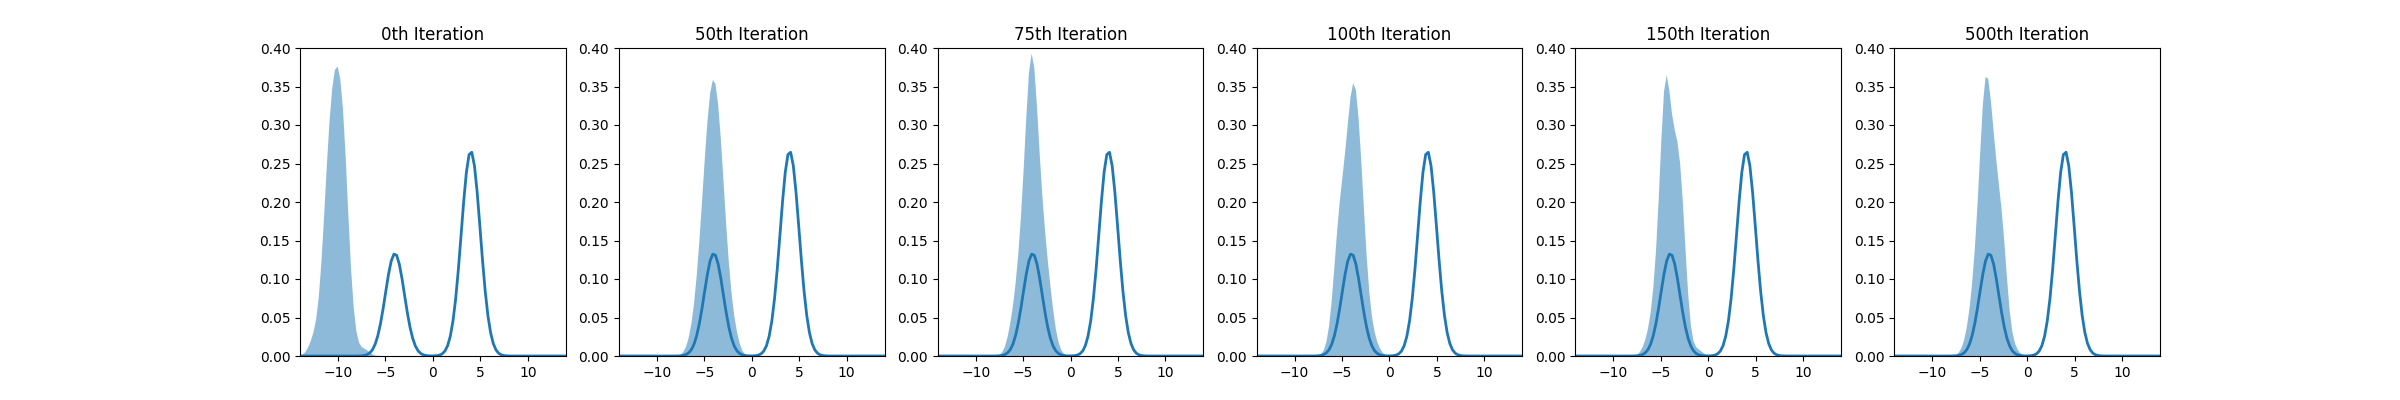
\includegraphics[width=\textwidth]{figs/toy-figure1_step0.25_mu4.0_w0.33_gaussian.png} \\
    %     \small (5) StepSize = 0.25, $\mu = \pm 4$, $(w_1, w_2) = (0.33, 0.67)$
    % \end{tabular}
    
    \begin{tabular}{@{}c@{}}
        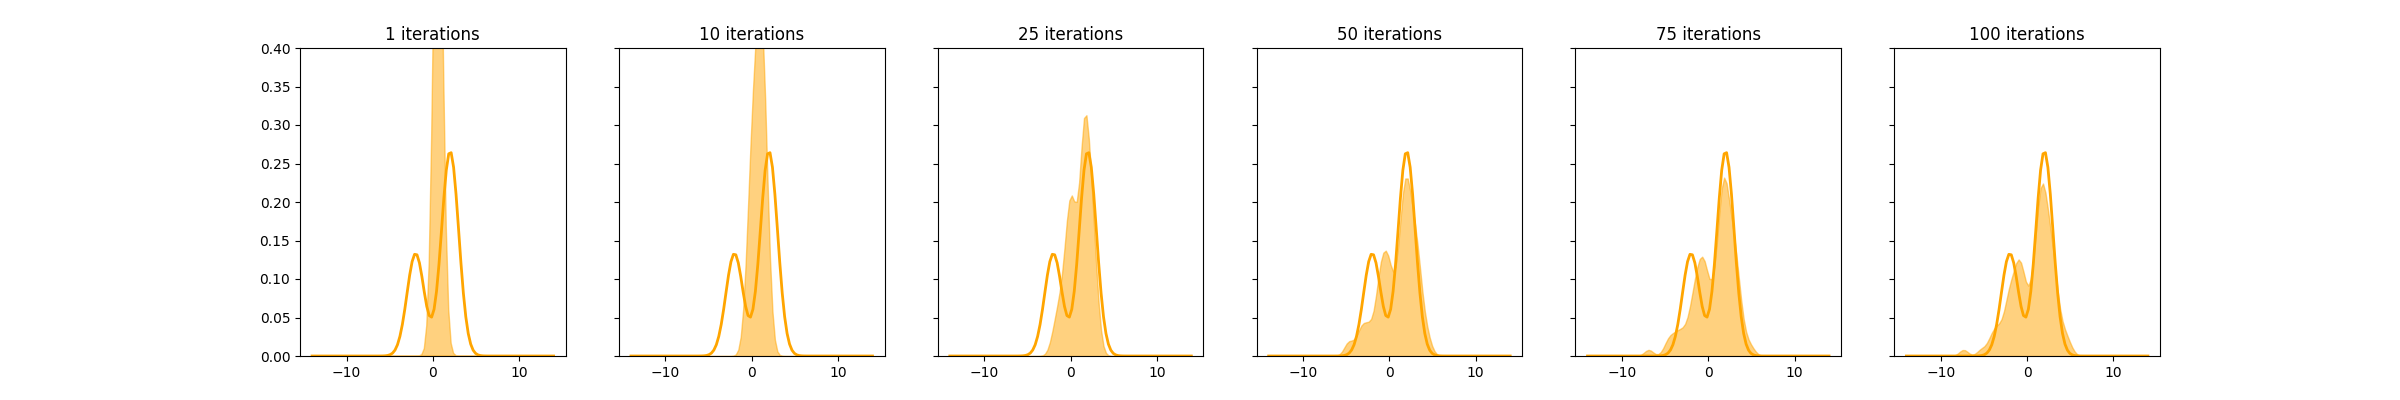
\includegraphics[width=\toyfigwidth]{figs/toy-figure1-numpyro.png} \\
        \small (4) ELBO Loss (NumPyro) StepSize = 0.1, 100 iters, $\mu = \pm 3$, $(w_1, w_2) = (0.33, 0.67)$
    \end{tabular}
     
    \caption{Toy example with 1D Gaussian mixture. Particle densities are visualized by KDE.}
    \label{fig:toy1dgaussian}
\end{figure}


\noindent\textbf{Illustration of the Convergence of SVGD}

We first reproduced the toy example about 1D Gaussian mixture mentioned in the paper. The task is to use SVGD to approximate a target distribution with PDF $p(x) = \frac{1}{3} N(x; -2, 1) + \frac{2}{3} N(x; 2, 1)$. The particles are initialized by an i.i.d. sample from the distribution $N(-10, 1)$, which is far away from the mode of the target distribution. We use 100 particles and 500 iterations with step size 0.25. We shown in figure \ref{fig:toy1dgaussian}, that SVGD effectively recovered the mixture distribution in $500$ epochs, as in Figure 1. (1)

We perform additional experiments for two other Gaussian mixture distribution: $\frac{1}{3} N(x; -3, 1) + \frac{2}{3} N(x; 3, 1)$ (where the two modes are farther apart) and $\frac{2}{3} N(x; -3, 1) + \frac{2}{3} N(x; 3, 1)$ (where the smaller mode is farther from the initialization distribution). We see that when the two modes are far apart from each other, the SVGD algorithm converges more slowly, as in Figure 1. (2). Moreover, when the smaller mode is far away from the initialization distribution, the particles in the SVGD algorithm have difficulty visiting the smaller mode, within 500 iterations, as in Figure 1. (3). We also replace the weighted negative log likelihood (over $n$ particles) in the SVGD Algorithm, with a single loss function that captures the $f$-divergence between the discrete particles and the target distribution p(x), such as ELBO. This ELBO-within-Stein algorithm is implemented NumPyro, and we found that when applying it to Gaussian mixture, the particles seem to converge faster and only need 100 iterations, as in Figure 1. (4).

\noindent\textbf{Illustration of the Performance and Scalability of SVGD}

The paper also found that SVGD performs better than Monte Carlo sampling on some expectation estimation tasks (smaller MSE). We implement this experiment based on our implementation of the toy example. We use both SVGD and MC to get samples/particles in the same size and check averaged MSE of three estimators estimating $E[X]$, $E[X^2]$, and $E[cos(\omega x + b)]$ respectively. We follow the same setting as in the original paper, except that we calculate averaged MSE over 400 runs for each setting. The results confirmed the claim in the paper, as shown in figure \ref{fig:toy1dmc}.

\begin{figure}[!htbp]
    \centering
    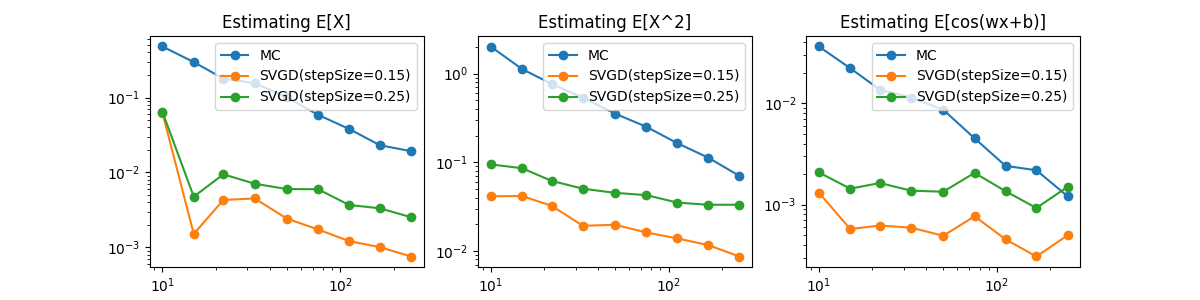
\includegraphics[width=\textwidth]{figs/toy-figure2-merged.png}
    \caption{Comparison between MC and SVGD on simple mean estimation tasks. }
    \label{fig:my_label}
\end{figure}


We observe that while SVGD performs better than MC, it is significantly slower. To know how scalable it is with large number of particles, we did an additional experiment (which doesn't exist in the original paper) to plot execution time of using different number of particles to match an unknown multivariate Gaussian in 1000 iterations. We implement two versions of the code, one using the original SVGD implementation in the paper, the other using NumPyro's SteinVI API with ELBO loss. We vary the number of particles from 100 to 1600. We found that the 
running time is quadratic with the number of particles, as shown in figure \ref{fig:timingparticles}.

\begin{figure}[!htbp]
    \centering
    \begin{tabular}{@{}cc@{}}
            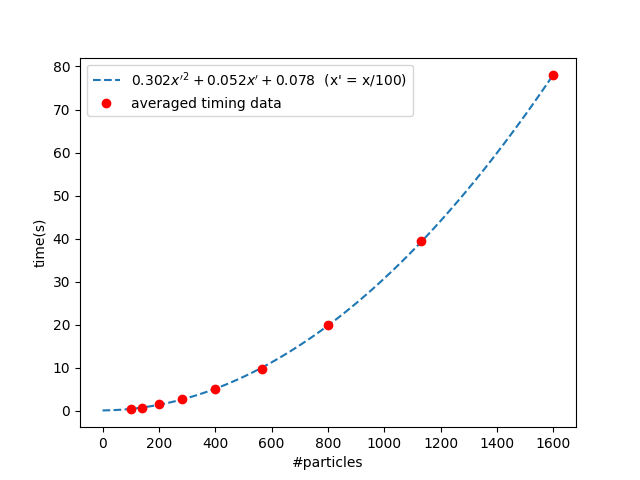
\includegraphics[width=0.40\textwidth]{figs/toy-timing-particles.png} & 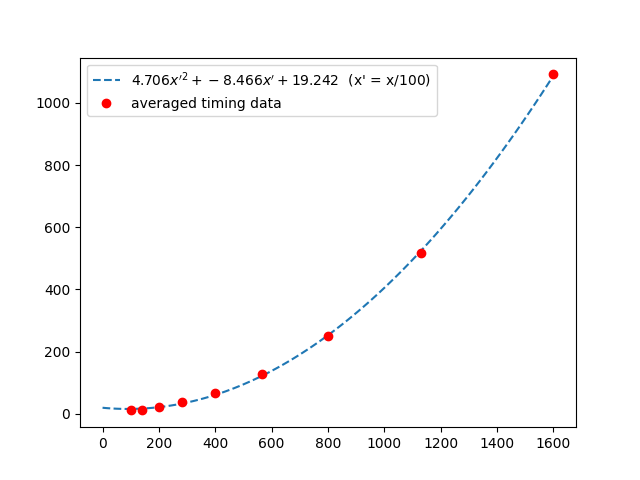
\includegraphics[width=0.40\textwidth]{figs/toy-timing-particles-numpyro-elbo.png}\\
        \small Original SVGD & NumPyro (ELBO Loss) \\
    \end{tabular}
    \caption{Timing vs particles }
    \label{fig:timingparticles}
\end{figure}


\subsection{Bayesian Logistic Regression}
\subsubsection{Small scale}
We attempt to test the SVGD algorithm in small-scale (less than $10^4$ data points) logistic regression tasks. We aim to construct a model which is able to predict a binary label of some training data. We run the SVGD algorithm as implemented on NumPyro against the No U-Turn Sampler (NUTS) algorithm \cite{nuts}. Both of the algorithms have implementations on NumPyro. Therefore for our experiments, we constructed a model representing the logistic regression problem using NumPyro primitives, and let NumPyro perform the inference process using the algorithms specified. The result is shown in Figure \ref{fig:logist_small}. We can see that the performance is about the same between both algorithms, but SVGD requires fewer particles to represent the distribution. 

\begin{figure}[h]
    \centering
    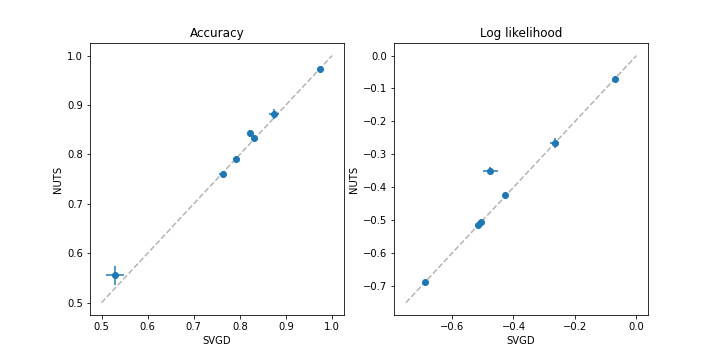
\includegraphics[width=0.6\textwidth]{figs/logistic_svgd_nuts.png}
    \caption{Comparison of accuracy (left) and log-likelihood (right) obtained by NUTS and SVGD algorithm on small-scale logistic regression dataset. The dotted line represents the situation where both algorithms perform as well was each other, and each point represent the average result on one of the dataset.}
    \label{fig:logist_small}
\end{figure}

\subsubsection{Large scale}
We also attempt to compare the performance of SVGD with other optimization algorithms on large scale Bayesian logistic regression in terms of test accuracy with respect to the number of iterations and particle size. We use the same dataset the original paper used, which is the binary Covertype dataset. The dataset contains 581012 data entries and each data point has 54 features. The binary Covertype dataset is a special variant of the original Covertype dataset which has 7 output classes. The binary version combines two output classes out of the 7 into class 1, and treats the rest classes as class 0. This dataset is very large even for current computers. If we do not use stochastic gradient descent and load all data in one batch, we would most likely encounter memory overflow. 

The baseline we choose is stochastic gradient Langevin dynamics (SGLD) \cite{ref_sgld}, where a noise term is added to the gradient in each step. In particular, we use the parallel version of SGLD. Fig \ref{fig:covertype} shows the evolution of test accuracy against training iterations and number of particles. Fig \ref{fig:acc_iter} compares the test accuracy between SVGD and SGLD when both of them are training for 2 epochs (roughly 18,000 iterations). SVGD consistently outperforms SGLD, achieving higher accuracy after 1000 iterations than SGLD after 18,000 iterations. However, from our experiments, the training using SVGD is far noisier than SGLD, which was not observed in the original experiments. Fig \ref{fig:acc_par} compares the test accuracy between SVGD and SGLD when the particle size varies. For each particle size, we conduct 50 independent trials and report the average performance. Similar to Fig \ref{fig:acc_iter}, the curves are not as smooth as the original plot. However, the relative performance still holds: SVGD is more particle efficient than SGLD, which means we can afford to reduce the number of particles to save more time in training.
\begin{figure}[ht]
	\centering
	\begin{subfigure}[b]{0.45\textwidth}
		\centering
		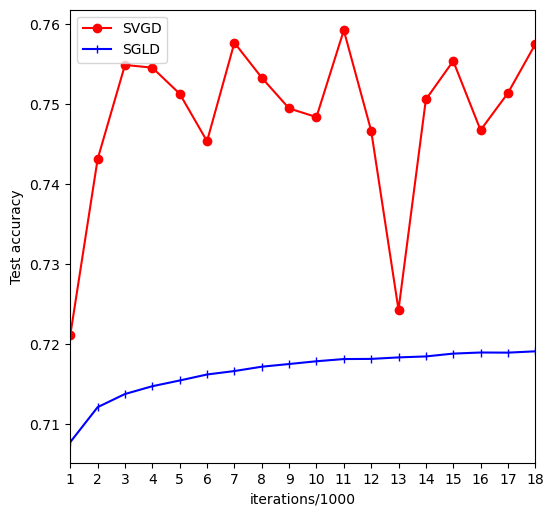
\includegraphics[height=0.2\textheight]{figs/sgvd_sgld_1.png}
		\caption{Test accuracy against every 1000 training iterations}
		\label{fig:acc_iter}
	\end{subfigure}
	\hfill
	\begin{subfigure}[b]{0.45\textwidth}
		\centering
		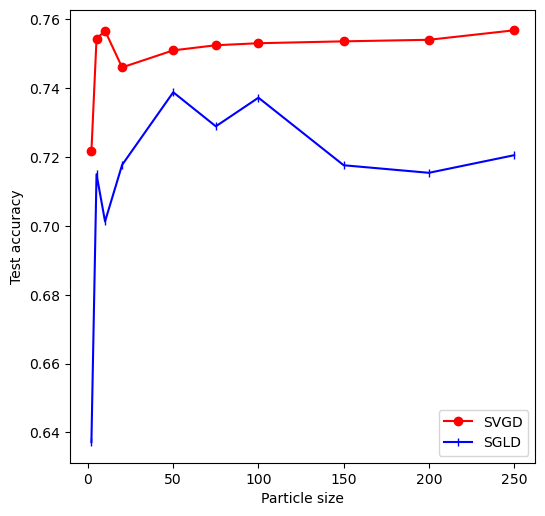
\includegraphics[height=0.2\textheight]{figs/sgvd_sgld_2.png}
		\caption{Test accuracy against number of particles at 3000 iterations ($\frac{1}{3}$ epochs)}
		\label{fig:acc_par}
	\end{subfigure}
	\caption{Results on Bayesian logistic regression on binary Covertype dataset for SVGD and SGLD. Left: Test accuracy against every 1000 training iterations. One epoch is roughly 9000 iterations given the batch size of 50. The number of particles used is 100. Right: Test accuracy against number of particles after 3000 training iterations are done. Experiments are done with 2, 5, 10, 20, 50, 75, 100, 150, 200, 250 particles. The dataset is divided into training and test set with a 8:2 ratio. Each experiment is done on 50 independent trials and the average number is reported.}
	\label{fig:covertype}
\end{figure}

\subsection{Bayesian Neural Network}

A Bayesian Neural Network (BNN) is a neural network where rather than finding the single optimal estimation for the model weights, we perform inference to find a posterior distribution for the model weights.

For the experiments, we train a small BNN on a set of regression tasks. We follow the setup from the paper and use the UCI dataset. The BNN trained has one hidden layer and has 50 units, except for the Protein dataset which instead uses a model with 100 units due to the higher data count. The training is done with subsampling size of 100.

We run tests on the SVGD algorithm as implemented by the authors of the original paper and also the implementation on NumPyro, and compare the performances against the probabilistic back-propagation (PBP) algorithm \cite{pbp}. One change made for the algorithm is to use the same number of epochs across all algorithms. For the Kin8nm, Naval, Power and Protein dataset, 50 epochs are used. The remaining dataset is trained on 200 epochs. The other hyperparameters were kept the same as the original code. Each experiments were repeated 10 times, except for the Protein dataset which was only repeated 5 times. We report the root-mean-squared error (RMSE) and the log-likelihood values of the test data in Tables \ref{tab:bnn}. 

\begin{table}[]
    \centering
    \resizebox{\textwidth}{!}{
    \begin{tabular}{|c|ccc|ccc|}
    \hline
     & \multicolumn{3}{|c|}{Average RMSE} & \multicolumn{3}{|c|}{Average log-likelihood} \\
     \hline
    Dataset & PBP & SVGD (original) & SVGD (NumPyro) & PBP & SVGD (original) & SVGD (NumPyro) \\
        \hline
    Boston & $3.007 \pm 0.278$ & $2.987 \pm 0.341$ & $3.290 \pm 0.369$ & $-2.879 \pm 0.261$ & $-2.689 \pm 0.158$ & $-2.809 \pm 0.043$ \\
    Concrete & $5.435 \pm 0.075$ & $5.240 \pm 0.134$ & $5.567 \pm 0.158$ & $-3.150 \pm 0.022$ & $-3.099 \pm 0.032$ & $-3.249 \pm 0.014$ \\
    Energy & $1.147 \pm 0.046$ & $0.890 \pm 0.032$ & $1.706 \pm 0.051$ & $-1.583 \pm 0.033$ & $-1.309 \pm 0.036$ & $-2.654 \pm 0.004$ \\
    Kin8nm & $0.097 \pm 0.001$ & $0.101 \pm 0.001$ & $0.100 \pm 0.001$ & $0.913 \pm 0.011$ & $0.871 \pm 0.009$ & $0.793 \pm 0.004$ \\
    Naval & $0.006 \pm 0.000$ & $0.004 \pm 0.000$ & $0.003 \pm 0.000$ & $3.766 \pm 0.009$ & $3.993 \pm 0.022$ & $4.125 \pm 0.003$ \\
    Power & $4.132 \pm 0.046$ & $4.168 \pm 0.053$ & $4.627 \pm 0.055$ & $-2.839 \pm 0.011$ & $-2.850 \pm 0.014$ & $-3.219 \pm 0.005$ \\
    Protein & $4.668 \pm 0.009$ & $4.493 \pm 0.018$ & $4.655 \pm 0.014$ & $-2.960 \pm 0.002$ & $-2.923 \pm 0.005$ & $-2.995 \pm 0.005$ \\
    Wine & $0.638 \pm 0.014$ & $0.632 \pm 0.015$ & $0.651 \pm 0.014$ & $-0.986 \pm 0.028$ & $-0.968 \pm 0.021$ & $-1.074 \pm 0.033$ \\
    Yacht & $0.689 \pm 0.047$ & $3.656 \pm 0.282$ & $3.546 \pm 0.195$ & $-1.129 \pm 0.038$ & $-2.741 \pm 0.065$ & $-3.350 \pm 0.004$ \\
    \hline
    \end{tabular}
    }
    \caption{Average root-mean-squared error (RMSE) and log-likelihood on test data for each algorithms on different BNN tasks.}
    \label{tab:bnn}
\end{table}

In our results, we were able to show that SVGD performs better than the PBP algorithm. In most test cases used, we are able to show that the predictions from the SVGD algorithm is more accurate than that from the PBP algorithm, as measured by the root-mean-squared error of the prediction. 

However, we found that the SVGD algorithm implementation on NumPyro was not able to replicate the performance that the original SVGD algorithm was able to. This could be due to the fact that unlike the SVGD algorithm from the original paper, the SVGD algorithm on NumPyro is minimizing the loss based on the ELBO value, and not the true posterior probability. We also find that the two implementations require different tunings of the hyperparameters to obtain the best performances. While the original SVGD implementation tend to not find the minimum with step sizes larger than $10^{-3}$, for the NumPyro version we had to increase the step size to $10^{-2}$ to get the best performance. 

We also report the amount of time required to run the algorithms in Table \ref{tab:bnn_time} in Appendix \ref{ssect:bnn-time}. We find that the original SVGD algorithm requires the least amount of time to compute. We also see that the NumPyro implementation of SVGD runs slower than the original implementation of SVGD due to the sampling required in the ELBO estimation process. The amount of sampling required for the ELBO estimate could have been reduced, however at a cost of a worse estimate of the value. However, we do note that the ELBO estimation could have been also been run in parallel, which we have not done for our tests.

In addition to experiments from the original paper, we also try to train the BNN while varying the number of epochs the training runs for. We plot some of these sessions in Figure \ref{fig:bnn-epoch} in Appendix \ref{ssect:bnn-epoch}. We were able to see that in the experiments, the SVGD algorithm may sometimes converge slowly to the true posterior. This may be due to the lower learning rate, which have been set in order for the samples to converge, although at a cost of slower convergence. As a result, we see that the SVGD algorithm will likely outperform the PBP algorithm if trained on for long enough.

%
% ---- Bibliography ----
%
% BibTeX users should specify bibliography style 'splncs04'.
% References will then be sorted and formatted in the correct style.
%
% \bibliographystyle{splncs04}
% \bibliography{mybibliography}
%
\begin{thebibliography}{8}
\bibitem{ref_article_svgd}
Liu, Q., Wang, D. (2016). Stein variational gradient descent: A general purpose bayesian inference algorithm. Advances in neural information processing systems, 29.

\bibitem{ref_lncs1}
Author, F., Author, S.: Title of a proceedings paper. In: Editor,
F., Editor, S. (eds.) CONFERENCE 2016, LNCS, vol. 9999, pp. 1--13.
Springer, Heidelberg (2016). \doi{10.10007/1234567890}

\bibitem{ref_book1}
Author, F., Author, S., Author, T.: Book title. 2nd edn. Publisher,
Location (1999)

\bibitem{ref_proc1}
Author, A.-B.: Contribution title. In: 9th International Proceedings
on Proceedings, pp. 1--2. Publisher, Location (2010)

\bibitem{ref_url1}
LNCS Homepage, \url{http://www.springer.com/lncs}. Last accessed 4
Oct 2017
\end{thebibliography}
\end{document}
